% Straight up stealing preamble from Eli Holmes 
%%%%%%%%%%%%%%%%%%%%%%%%%%%%%%%%%%%%%%START PREAMBLE THAT IS THE SAME FOR ALL EXAMPLES
\documentclass{article}

%Required: You must have these
\usepackage{Sweave}
\usepackage{graphicx}
\usepackage{tabularx}
\usepackage{hyperref}
\usepackage{natbib}
\usepackage{pdflscape}
\usepackage{array}
\usepackage{gensymb}
%\usepackage[backend=bibtex]{biblatex}
%Strongly recommended
  %put your figures in one place
%\SweaveOpts{prefix.string=figures/, eps=FALSE} 
%you'll want these for pretty captioning
\usepackage[small]{caption}

\setkeys{Gin}{width=0.8\textwidth}  %make the figs 50 perc textwidth
\setlength{\captionmargin}{30pt}
\setlength{\abovecaptionskip}{10pt}
\setlength{\belowcaptionskip}{10pt}
% manual for caption  http://www.dd.chalmers.se/latex/Docs/PDF/caption.pdf

%Optional: I like to muck with my margins and spacing in ways that LaTeX frowns on
%Here's how to do that
 \topmargin -1.5cm        
 \oddsidemargin -0.04cm   
 \evensidemargin -0.04cm  % same as oddsidemargin but for left-hand pages
 \textwidth 16.59cm
 \textheight 21.94cm 
 %\pagestyle{empty}       % Uncomment if don't want page numbers
 \parskip 7.2pt           % sets spacing between paragraphs
 %\renewcommand{\baselinestretch}{1.5} 	% Uncomment for 1.5 spacing between lines
\parindent 0pt% sets leading space for paragraphs
\usepackage{setspace}
%\doublespacing

%Optional: I like fancy headers
%\usepackage{fancyhdr}
%\pagestyle{fancy}
%\fancyhead[LO]{How do climate change experiments actually change climate}
%\fancyhead[RO]{2016}
 
%%%%%%%%%%%%%%%%%%%%%%%%%%%%%%%%%%%%%%END PREAMBLE THAT IS THE SAME FOR ALL EXAMPLES

%Start of the document
\begin{document}

%\SweaveOpts{concordance=TRUE}
\bibliographystyle{..//..//refs/bibstyles/amnat.bst}% i moved a style file into the ospree git repo. feel free to add whatever style you like and update, lizzie! I don't have besjournals

\title{Supplemental materials  for Chilling outweighs photoperiod and forcing cues for temperate trees in experiments, but not in natural systems} % perspective paper for OSPREE analyses
% or Chilling dominates tree budburst in controlled climate experiments, but not in the great outdoors

\author{A.K. Ettinger, C. Chamberlain, I. Morales-Castilla, D. Buonaiuto, D. Flynn, T. Savas, \\J. Samaha \& E. Wolkovich}
%\date{\today} 
\maketitle  %put the fancy title on
%\tableofcontents      %add a table of contents
%\clearpage
%%%%%%%%%%%%%%%%%%%%%%%%%%%%%%%%%%%%%%%%%%%%%%%%%%%


\section*{May need to move back to main text ...}

\par The paucity of studies directly manipulating chilling---which our results suggest has the greatest effect on budburst---suggests a major gap in current research. While many studies (X out of Y here) directly manipulated forcing, far fewer directly manipulated chilling (Z out of Y). 
% [Next bit is in main text currently.] Instead many studies (J out of Y) estimate chilling effects through sequential removal of tissue from the field and exposure to `forcing' conditions (cite Weinberger), with the assumption that tissue collected later experienced more chilling. The challenge with this method is that photoperiod and other factors have also changed during this time. Indeed, we found estimates varied in XX way when derived from direct manipulations of chilling versus the sequential `Weinberger' method. 
Our model highlights how the choice of chill units can affect model estimates and associated forecasts (reference supplemental figure with utah units vs chill portions in main manuscript). 
Given the limited manipulation of chilling in studies, we estimated chilling for all studies by combining chilling from the field (i.e., chilling before plants were sampled) and experimental chilling into two widely used metrics of chilling: Utah and Chill portions \citep{dennis2003}. We found the effects of chilling and other cues remain qualitatively consistent across the two chilling units, though chilling and photoperiod estimates were slightly lower using chill portions compared to Utah (cite supplemental table comparing estimates with both units).  % We could shorten this paragraph further. And then add something about how we need better models of chilling ...

% Note that we don't actually know if tissue is dormant, so we should not say dormant twigs ....
%Most studies do not experimentally apply chilling by manipulating duration or temperature of chilling, nor do most estimate the chilling imposed in their experiment. We therefore calculated the chilling imposed by most studies, as it would otherwise have been impossible to provide estimates with only experimental chilling (reference lizzie's supp heat maps). %this last part may be better for methods?

\par An additional important limitation is the rarity of studies designed to test interactions. Interactions between these cues are widely expected (cites) and, when examined, often found (cites), we were unable to estimate interactions in our meta-analysis because very few studies design experiments to test for interactions between chilling, forcing, and photoperiod (cite table with number of interactions from coding challenge!). The few that do incorporate interactions generally use the Weinberger method, which is not designed to robustly tease out of the effects of multiple cues (cites, Tables, figs).  Our estimated effects average over interactions \citep{gelman2006}, but identifying them in future research will be critical to understanding and predicting budburst. For example, the most commonly observed interaction between chilling and forcing---that lower amounts of chilling increases forcing requirements for budburst %\citep{} 
(cite papers in the ospree database that interact chilling and forcing)
---is the hypothesized cause of declining sensitivities in European trees \citep{fu2015,vitasse}. As more data become available, it would allow additional tests of important interactions, such as how responses vary across latitudes (ref latitude figure). % Maybe add: In addition to data limitation, disentangling forcing from chilling conditions is a challenge because information on endodormancy requirements is very scarce \citep{chuine2016}.% Though I wonder if this belongs above in discussion of chilling?

\section*{Things we'd like to discuss in main paper but don't have room for}

% I suggest we save a discussion of Photothermoperiodicity for a plant-specific journal in which we have a much larger number of words ...
\par \underline{Photothermoperiodicity}, for example, is an ongoing challenge: chamber studies may seek to replicate patterns in nature, pairing daylength and temperature treatments such that night temperatures are always cooler than day temperatures (e.g., cite studies that do this).  This results in daylength treatments that differ in temperature conditions (and therefore chilling and forcing treatments) as well, however.  

\par \underline{Chilling:} Current common models for chilling (i.e., Utah which was developed for XX species,  chill portions which was developed for XX species) are \emph{hypotheses} for how chilling may accumulate to affect the process of dormancy release, but are likely to be inaccurate for many species. Our model highlights how the choice of chill units can affect model estimates and associated forecasts (Figures 1,\ref{fig:figmucpz}\ref{fig:muutnonz}, \ref{fig:mucpnonz}). 

\
\section*{Supplemental Methods}
% Include:
% Why we studied budburst and what it means ... Cat put together a 'what is budburst' file we should include with database. (Full OSPREE: 13,000 rows across 85 studies across 41 years and 227 species)

\begin{enumerate}
\item Data: search terms, etc
\item Species complex description
\item Equation of our model

\item Quick review of what standardized units are (We used a standardized scale to allow comparisons of the three cues ...)

\item Forecasting with the OSPREE model: We selected sites in Germany where temperature and budburst have been monitored since the 1950s. We extracted mean temperature data from 1951 through 1961 (pre warming time period) and used these values as baseline data. We then investigated model predictions of budburst given different levels of warming (from 1-7 \degree C) above this baseline, including altered chilling and forcing as well as potential declines in photoperiod due to advancing phenology. We did this for one common European species: \emph{Betula pendula} (silver birch) at all lat/longs included in the PEP database between 1951 and 1961. We also did this for another common European species, \emph{Fagus sylvatica}, for a subset of sites where it occured with \emph{B. pendula}, in order to compare budburst responses of these two species when they experience the same baseline climate and warming levels.

\item  To understand how experimental temperature, photoperiod, and budburst sensitivity compares to past and current conditions in nature, we used data from the PEP database (cite). We summarized forcing, chilling, and budburst doy for two common species: \emph{Betula pendula} (silver birch) and \emph{Fagus sylvatica} (European beech) during a pre-warming time-period (1950-1980) and post-warming period (1981-2014?). 

\end{enumerate}
\section*{Supplemental Results/Discussion}
\begin{enumerate}
\item Surprising species-specific responses: 
\begin{enumerate}
\item Positive Responses to chilling for Tilia and Salix.  have positive response to chilling with chill portions model. T

\item Poisitive responses to forcing: Acer-complex, Fraxinus complex, Cornus alba.
\end{enumerate}
\end{enumerate}

\section*{Supplemental Tables}
\begin{enumerate}
\item Table 1S: Species included in OSPREE, with the reference(s) of studies they are included in, the range of forcing, chilling, and photoperiod treatments in these studies, and perhaps the range of latitudes.
\item Table 2S: model estimates for 4 models: Utah z (used in main text Figure 1), Utah uncentered, Chill portions z, Chill portions uncentered
\item Table 3S: a table that goes with Figure 3 (the 4-paneled 3D forecasting figure) that includes the mean budburst day of year, chilling estimates, mean winter temperature, and spring (forcing) temperatures for the 4 sites with no warming and with the 7 levels of warming.
\end{enumerate}
\section*{Supplemental figures}
\begin{enumerate}
\item Map of study locations, shading or symbol coding for number of cues (Lizzie)
\item Map of species forecasting to justify sites
\item Heat maps for the main data associated, including by actual study design and by calculated chilling (our calculations)
\item Photoperiod x latitude effects figure
\item Maps of current and forecasted budburst and chilling for PEP sites (heat maps)


\end{enumerate}


\section*{Understanding declines in temperature sensitivity in European long-term data}
% See files: PEP_climate/comparetopepsims.R and pep_sims/pepvarsim.R 
% HELP from Cat needed !!! I guessed at the methods for PEP sites ... She should double-check everything I wrote
As our model results (when applied to realistic forcing, chilling and photoperiod conditions in Europe) do not predict a dramatic decline temperature sensitivity, we tested whether observed declines could instead be due to a statistical artifact of the method commonly used to estimate temperature sensitivity (a linear regression of annual budburst date versus mean or other aggregated metrics of spring temperature yielding estimates in days/$^{\circ}$C). If warming produces systematically warmer daily temperatures this method will inherently estimate lower sensitivities, because the `days' unit will effectively have increased in the thermal time it represents.

\par To test this hypothesis we compared observed trends with simulations. First, we collated PEP 725 (CITE) data for \emph{Betula pendula} for all sites with leafout data each year from two 10-year time-periods: 1950-1960, which represented a period before significant anthropogenic warming (citeIPCC) and 2000-2010, a period with significant warming. We used leafout data (BBCH=XX) instead of budburst (BBCH=XX) as leafout data are far more common in the PEP 725 database. Next, we simulated budburst data with constant cues. For this, we did not include any chilling or photoperiod cues, but simply assumed budburst occurred after a certain summation of heat, estimated via growing degree days with a base temperature of 0$^{\circ}$C. We then estimated temperature sensitivity (days/$^{\circ}$C)) and the difference in these estimates given different levels of spring warming. For the simulations showed here we used a GDD requirement of 150, a base mean spring temperature of 6$^{\circ}$C with a variance of 3$^{\circ}$C and estimated temperature sensitivity for 10-year periods for 45 simulated sites (these values were chosen to best match the PEP 725 data, but note that the general findings are robust to other combinations of these parameter values).

\par As expected temperature sensitivity estimates for \emph{Betula pendula} from PEP 725 declined across the two time periods in step with warming daily temperatures. Across the sites studied here we estimated a decline of 0.9$\pm$0.3 days/$^{\circ}$C (comparing 2000-2010 and 1950-1960) and 1.1$^{\circ}$C warming; this estimate was very similar to simulations given constant cues and 1$^{\circ}$C warming (Fig. \ref{fig:pepsims}). Additionally, in both the real and simulated data variance in leafout date declined, as would be expected if plants use a thermal sum threshold of forcing to leaf out and warming produces systematically warmer days: in the PEP 725 data we found a decline in leafout variance of 57\%, compared to a decline of 37\% in the simulations. Additionally we found little change in accumulated chilling (1 September - 1 March of each year) in the PEP 725 data across the two time points (2247$\pm$31 Utah units in 1950-1960, compared to 2236$\pm$20 Utah units in 2000-2010), further suggesting that shifts in chilling do not explain the declining sensitivities. Simple plots of the chilling and forcing required for budburst suggest very low chilling is often required to dramatically increase the forcing required for budburst (Fig. {fig:pepgddchill}).
% Need to add SE or such to % ... See PEP_climate/comparetopepsims.R




\section*{Reference list}

A few categories:\\

Papers about contrasting results over what cues matter from growth chamber studies: \cite{Basler:2012,Basler:2014aa,Caffarra:2011qf,Caffarra:2011a,Caffarra:2011b,Heide:2005aa,koerner2010b,Laube:2014a,vitasse2013,zohner2016}. Get Nanninga \emph{et al.} 2017: 'Increased exposure to chilling advances the time to budburst in North American tree species' and maybe Malyshev \emph{et al.} 2018 `Temporal photoperiod sensitivity and forcing requirements for budburst in temperate tree seedlings.'\\

Papers about declining sensitivities (Ailene will update this list): \cite{Rutishauser:2008,fu2015}. Also look for a Wang \emph{et al.} article `Impacts of global warming on phenology of spring leaf unfolding remain stable in the long run.' Vitasse paper on declining variation across elevation gradient. See \cite{yu2010}, but this is not temperate trees. \\

Papers about chilling units paper (Lizzie gets a list): Fu 2012 from OSPREE. \cite{harrington2015}\cite{lued2011,Luedeling:2011qe,Luedeling2013AgFM}\\

\bibliography{..//..//refs/ospreebibplus.bib}

section* {Figures}

\newpage

\begin{figure}[h!]
\centering
\noindent 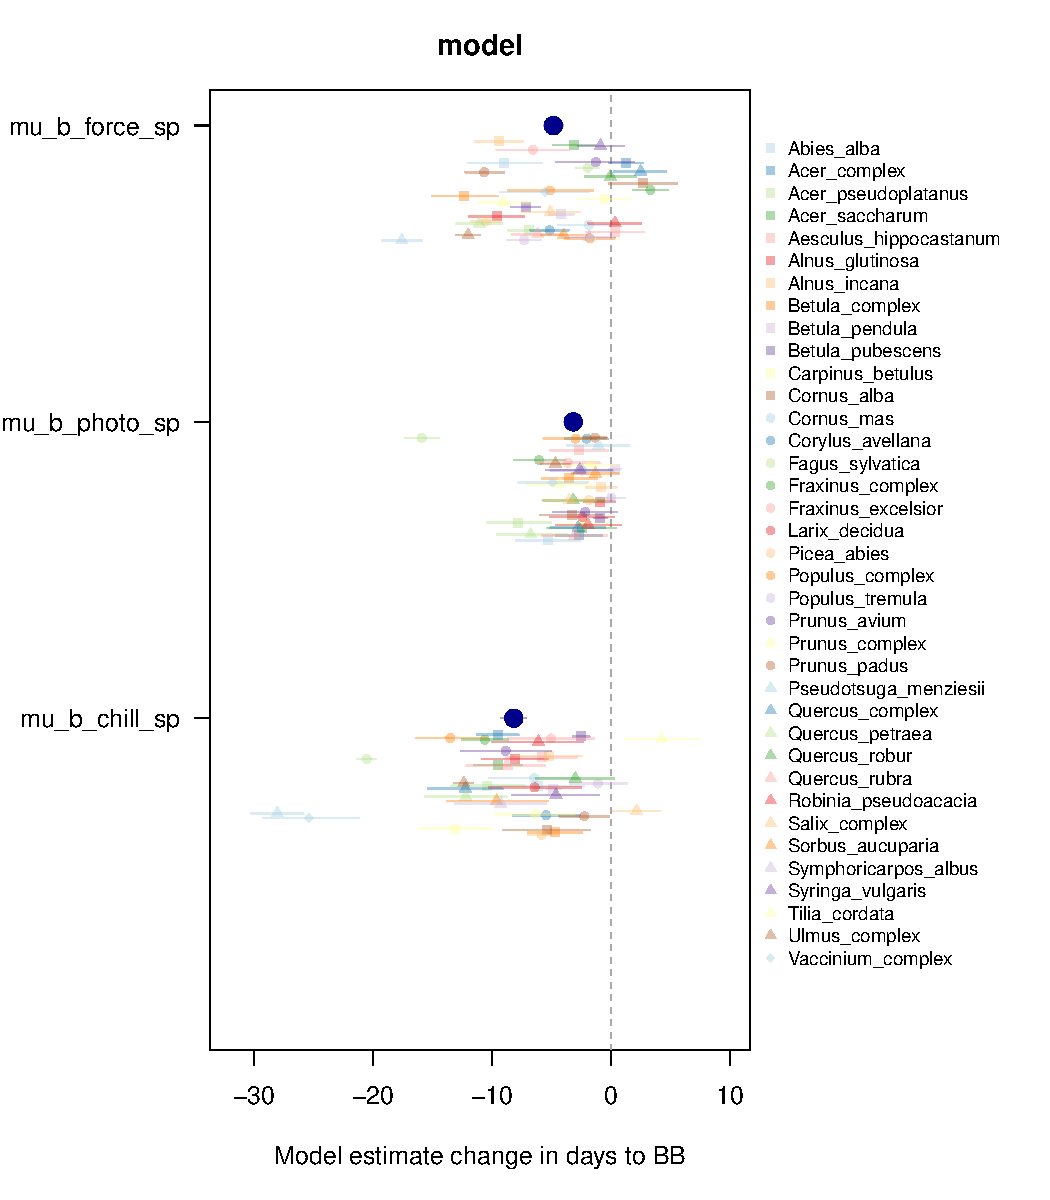
\includegraphics[width=0.75\textwidth]{..//..//analyses/bb_analysis/figures/muplotmodelspcompexprampfpcp_z.pdf}
\caption{\emph{Estimates for effects of chilling, forcing, and photoperiod from the model fit with Chill Portions}, with centered data, enabling comparisons of effect sizes across predictors. Coefficients were qualitatively similar to those in the model with Utah and can be found in the main text. Convert this into a table and combie with below figure!} 
\label{fig:mucpz}
\end{figure}

%no need for figure- just do below as a table
%\begin{figure}[h!]
%\centering
%\noindent 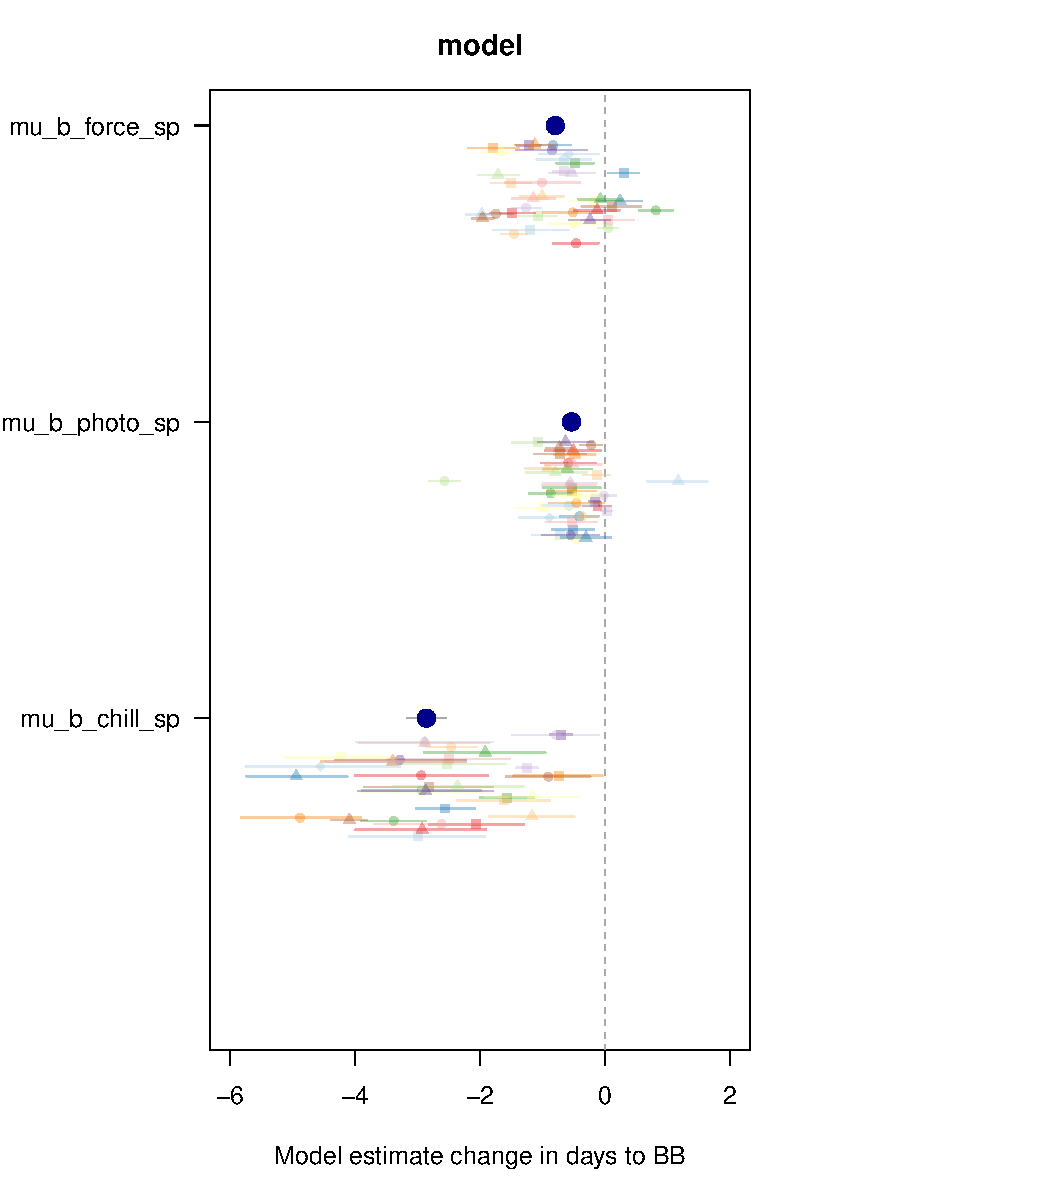
\includegraphics[width=0.75\textwidth]{..//..//analyses/bb_analysis/figures/muplotmodelspcompexprampfputah_nonz.pdf}
%\caption{\emph{Estimates for effects of chilling, forcing, and photoperiod from the models fit with uncentered predictors} using Utah units. Relationships of coefficients were qualitatively similar to those in the centered models (Figures 1, \ref{fig:mucpz}.} 
%\label{fig:muutnonz}
%\end{figure}
\begin{figure}[h!]
\centering
\noindent 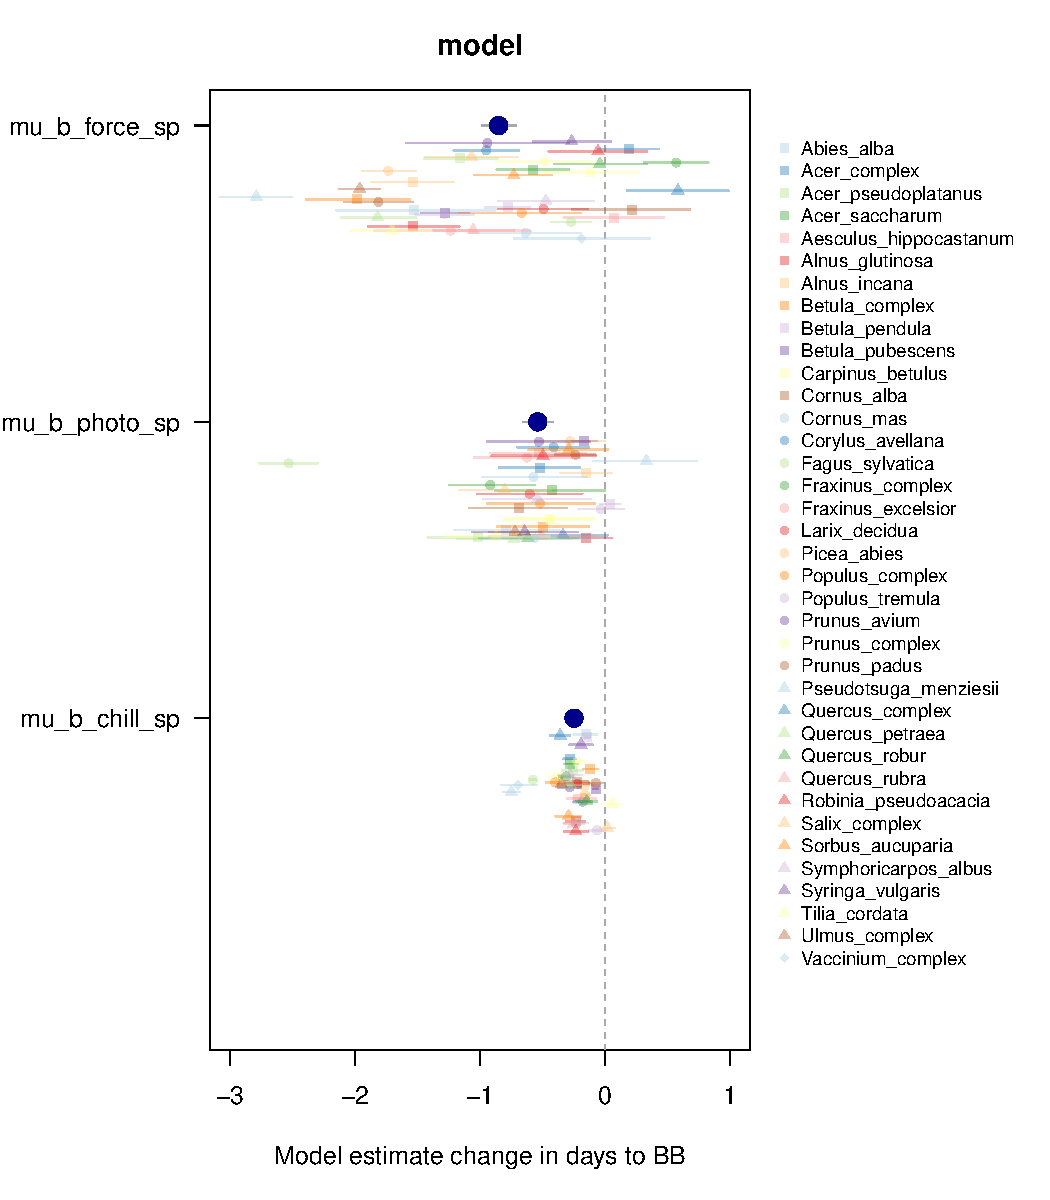
\includegraphics[width=0.75\textwidth]{..//..//analyses/bb_analysis/figures/muplotmodelm2lni_spcompexprampfpcp_nonz.pdf}
\caption{\emph{Estimates for effects of chilling, forcing, and photoperiod from the models fit with uncentered predictors} using Chill Portions. Convert this into a table and combie with above figure!} 
\label{fig:mucpnonz}
\end{figure}


\newpage
\begin{figure}[h!]
\centering
\noindent 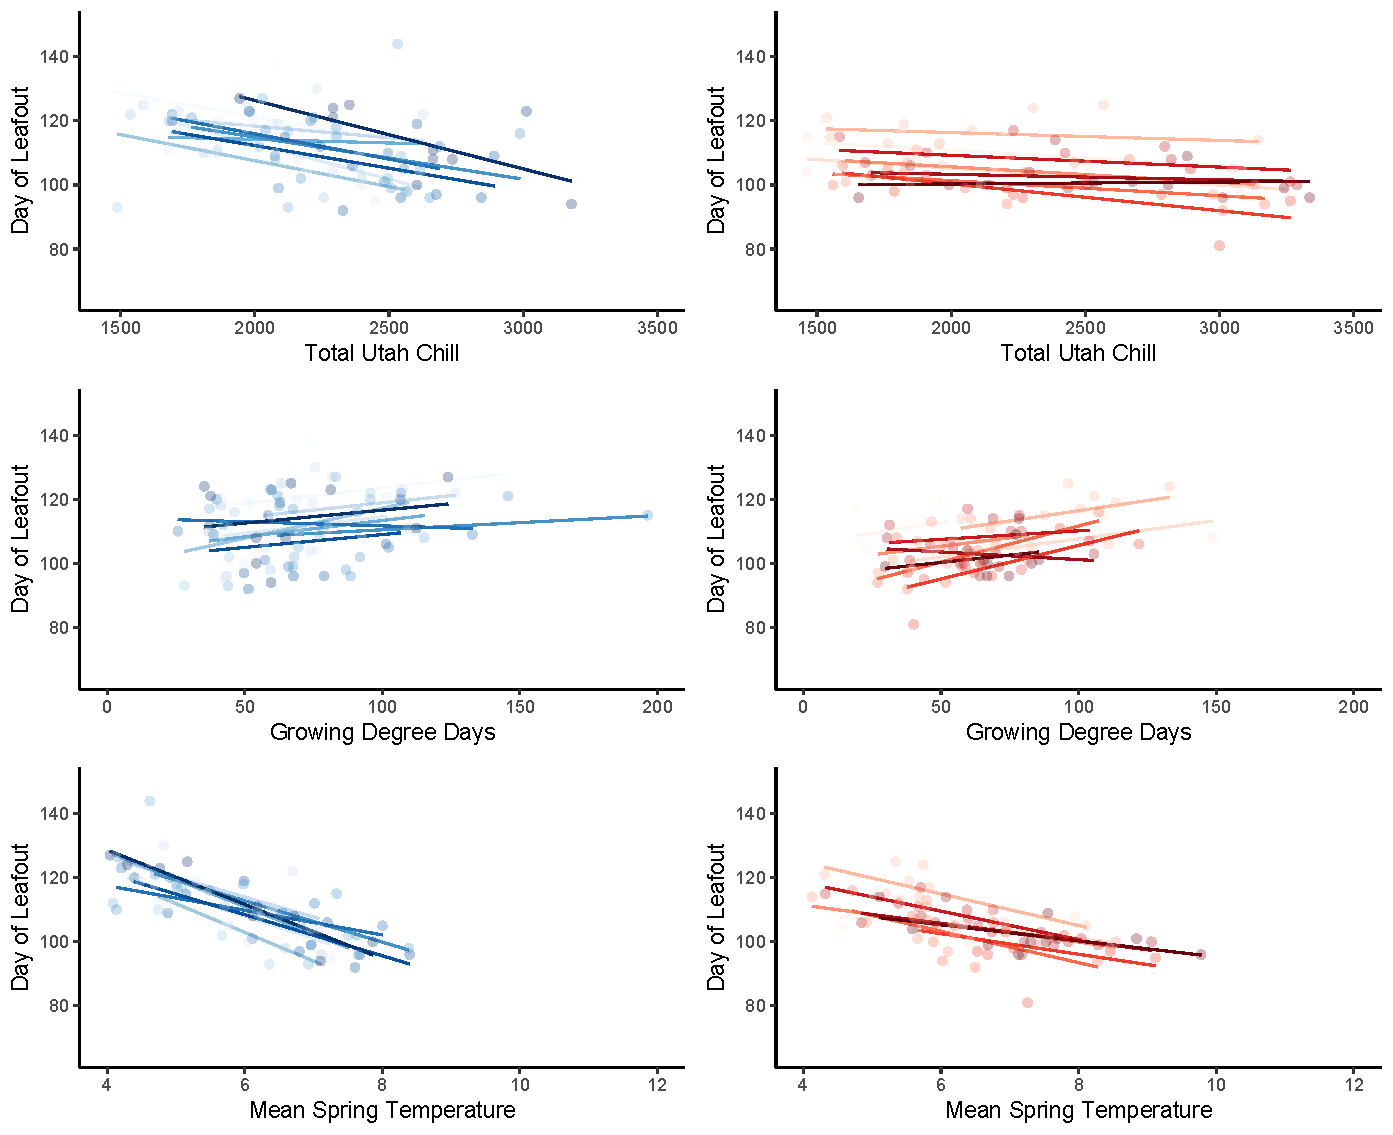
\includegraphics[width=0.75\textwidth]{..//..//analyses/bb_analysis/PEP_climate/figures/betpen_multruns_utahgddmat.pdf}
\caption{Day of leaf out versus chilling, growing degree-days, and mean spring temperature pre- (left panels, 1951-1961) and post- warming (right panels,1981-1991????) for PEP sites in Germany where \emph{Betula pendula} phenology has been monitored for decades.}
\label{fig:pep}
\end{figure}

\newpage
\begin{figure}[h!]
\centering
\noindent 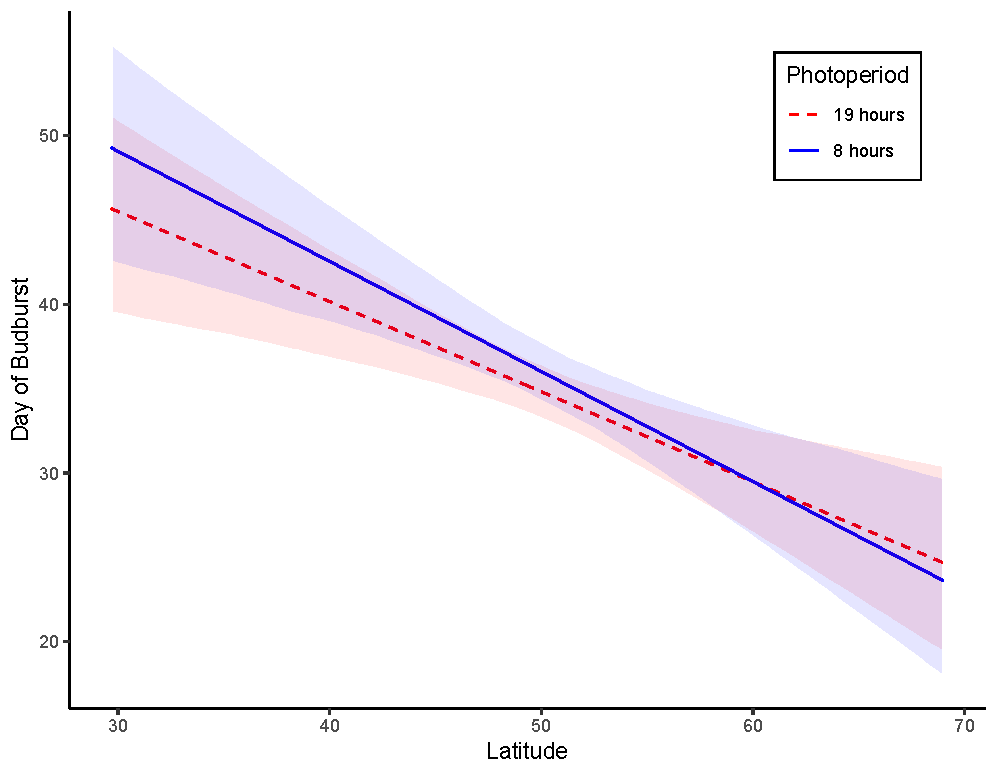
\includegraphics[width=0.75\textwidth]{..//..//analyses/lat_analysis/figures/LatxPhoto_allspp.pdf}
\caption{Latitude model. Cat: Could you make a muplot that is similar to those in the main text? Should we keep this plot, or something similar as a second panel?}
\label{fig:lat}
\end{figure}

\begin{figure}[h!]
\centering
\noindent 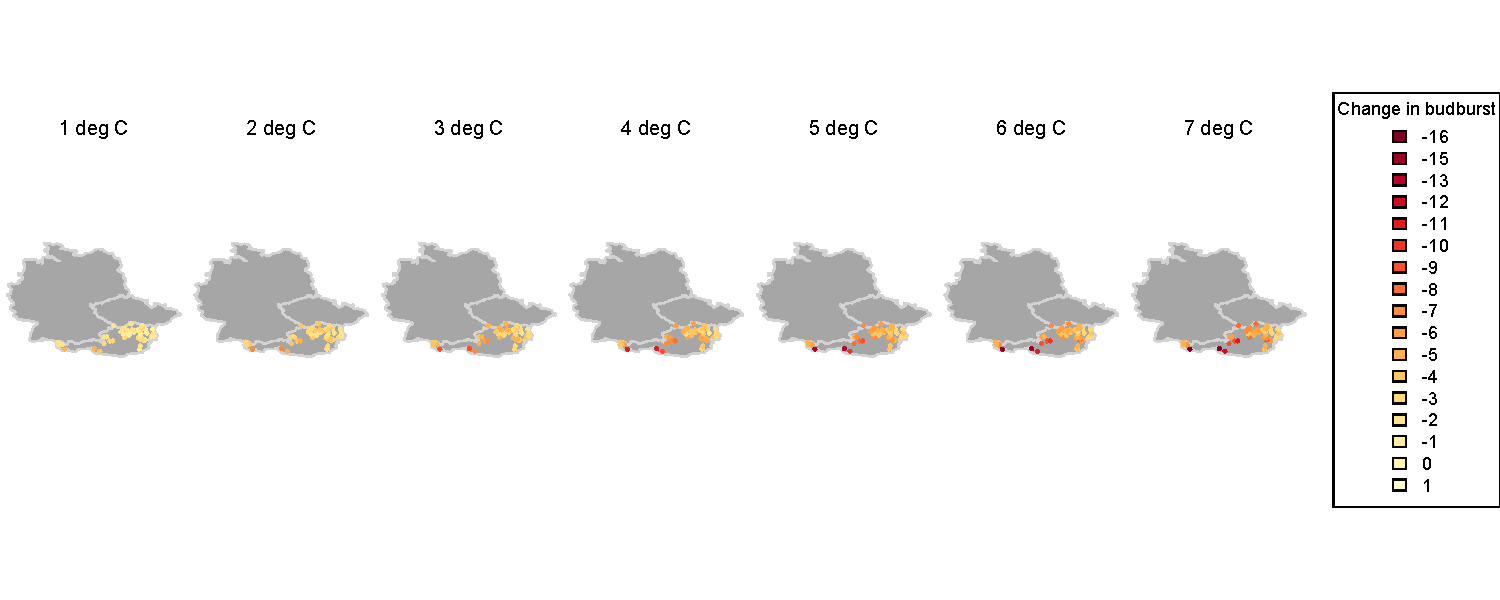
\includegraphics[width=0.75\textwidth]{..//..//analyses/bb_analysis/figures/forecasting/forecastbetpenPEPBB_map.pdf}
\caption{Forecasted chilling and budburst, in PEP areas. Ailene will update this. }
\label{fig:foremap}
\end{figure}
\begin{figure}[h!]
\centering
\noindent 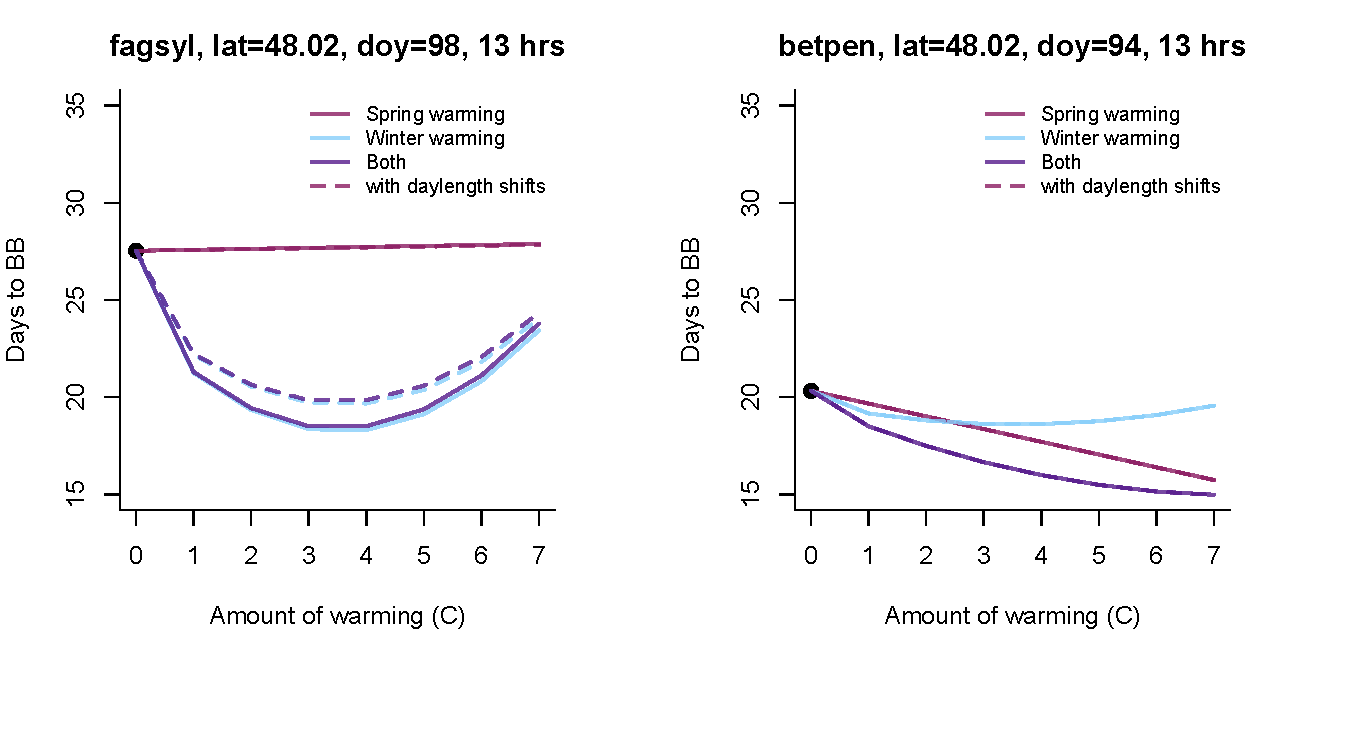
\includegraphics[width=0.75\textwidth]{..//..//analyses/bb_analysis/figures/forecasting/tempforecast_bothspp_PEPBB_wdl_utah.pdf}
\caption{Forecasted }
\label{fig:foremap}
\end{figure}


\newpage
\begin{figure}[h!]
\centering
\noindent 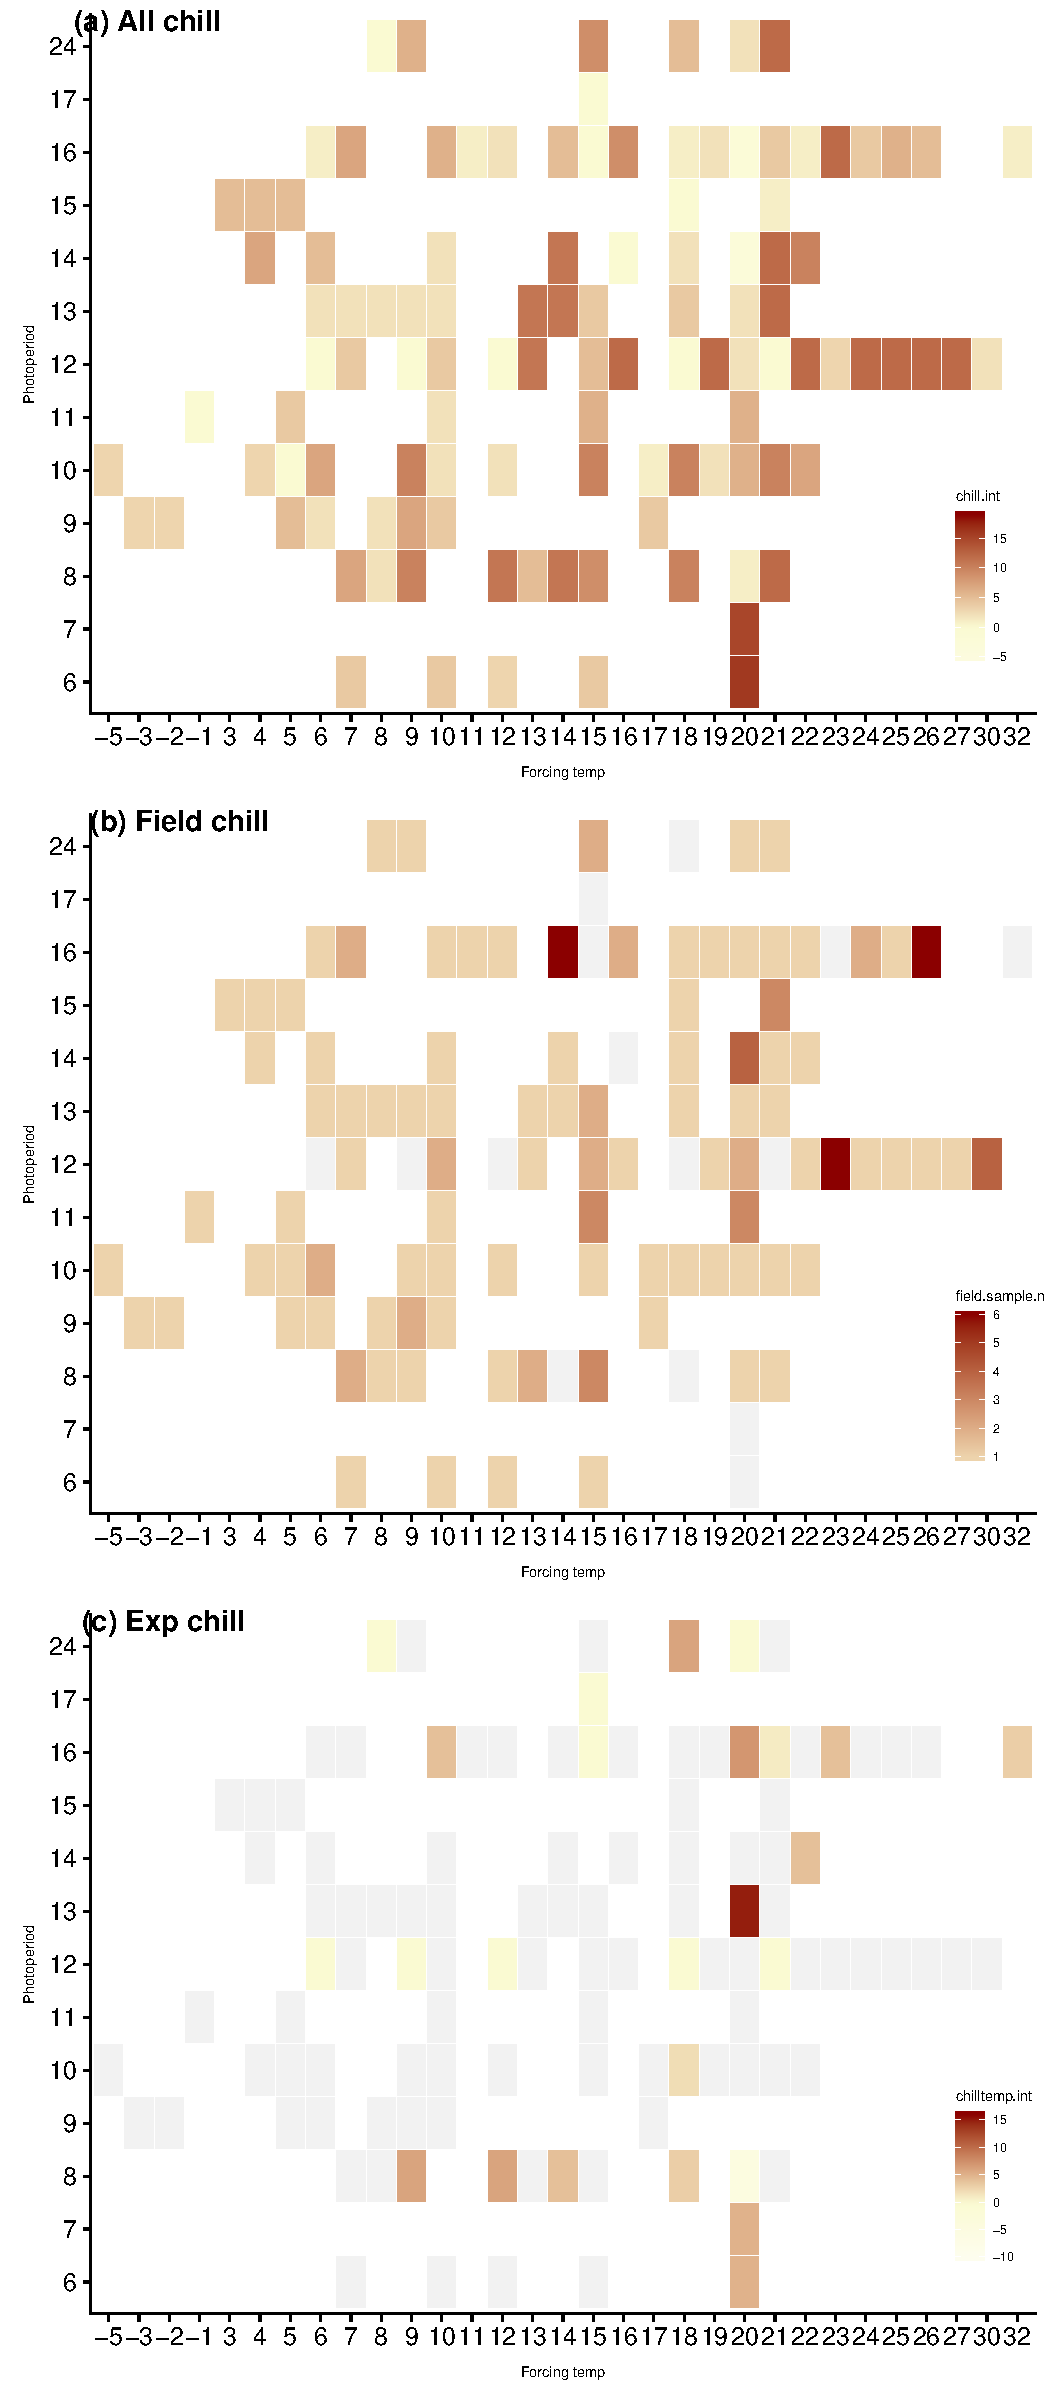
\includegraphics[width=0.75\textwidth]{..//..//analyses/bb_analysis/figures/studydesign_heat3panel.pdf}
\caption{Heatmaps of treatments ... need to make sure this matches the data we have ended up using!}
\label{fig:treatheatmaps} % see bb_analysis/studydesignplotsbb.R 
\end{figure}


\newpage
\begin{figure}[h!]
\centering
\noindent 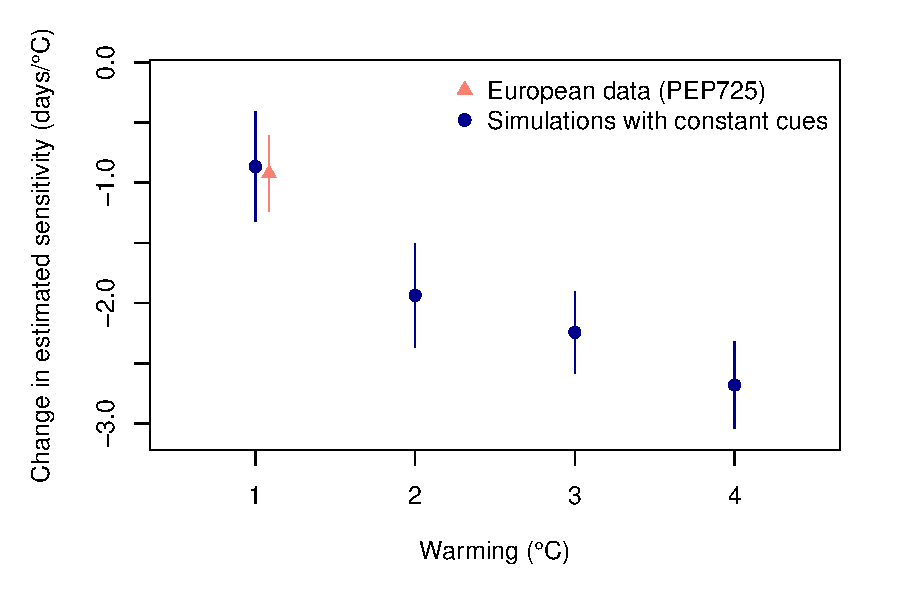
\includegraphics[width=0.75\textwidth]{..//..//analyses/bb_analysis/PEP_climate/figures/peprealandsims.pdf}
\caption{Declining sensitivities observed in long-term European data for a suite of common trees may be explained by a statistical artifact. We compared the sensitivity estimated from linear regressions of day of leafout versus mean spring temperature (estimated thus as days/$^{\circ}$C) from PEP 725 data for \emph{Betula pendula} from 45 sites (`European data') with estimated declines in simulations where the cues were held constant but spring temperatures warmed by 1-4$^{\circ}$C (`Simulations') and found the estimated temperature sensitivity measured as days/$^{\circ}$C declined even though the underlying cues had not changed, see \emph{Understanding declines in temperature sensitivity in European long-term data} in Supplement for further details.}
\label{fig:pepsims}
\end{figure}

\newpage
\begin{figure}[h!]
\centering
\noindent 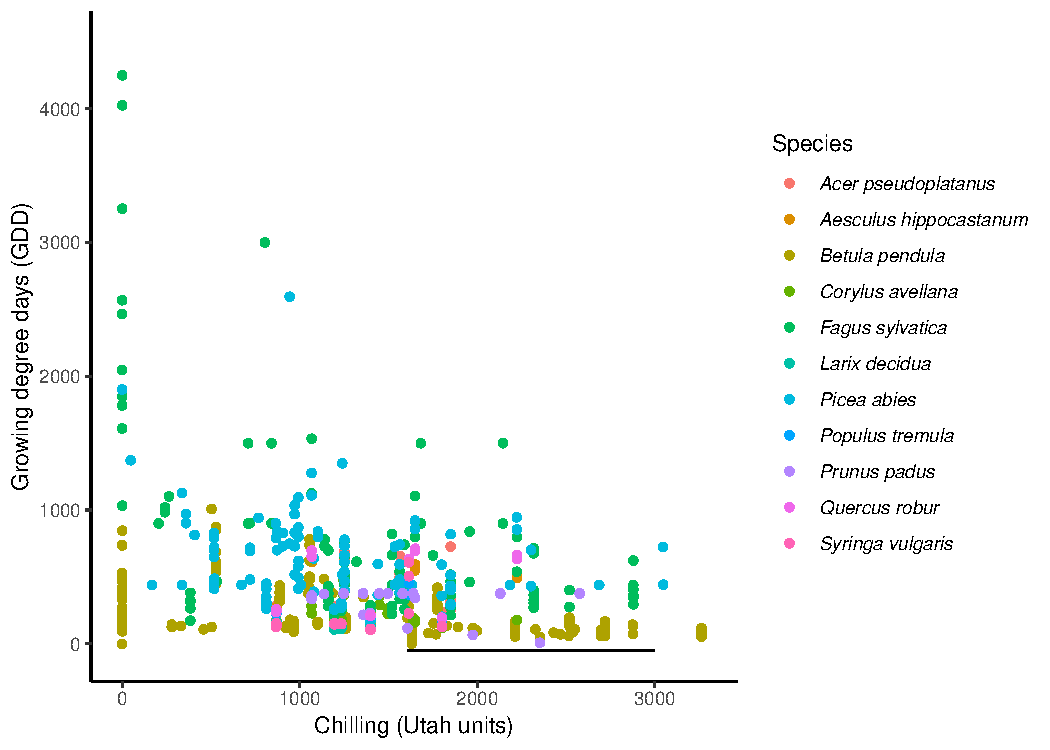
\includegraphics[width=0.75\textwidth]{..//..//analyses/bb_analysis/figures/gddbyutah_pepspp.pdf}
\caption{GDD (growing degree days) versus chill units at the time of budburst from the OSPREE database for common species in the PEP 725 long-term phenological database. The black line shows the range of chilling (10-90\% quantiles) accumulated from 1 September to 1 March for 45 sites for \emph{Betula pendula} (see also \emph{Understanding declines in temperature sensitivity in European long-term data}). We calculated GDD  here as the average daily forcing temperature multiplied by days to budburst. }
\label{fig:pepgddchill}
\end{figure}



%%%%%%%%%%%%%%%%%%%%%%%%%%%%%%%%%%%%%%%%
\end{document}
%%%%%%%%%%%%%%%%%%%%%%%%%%%%%%%%%%%%%%%%
